\chapter{Descripción de los problemas en fluidos con transferencia de calor }
\graphicspath{{figs/cap4/}}
\label{cap4}

En el presente capíulo se realiza la descripción de los problemas con transferencia de calor para fluidos multifásicos con cambio de fase llevados a cabo para validar el código numérico desarrollado, siendo éstos la \textit{Construcción de Maxwell} y la \textit{Estratificación de un fluido Van Der Waals}

\section{Construcción de Maxwell}

Como se desarrollo en el Cap. \ref{cap2} la Ec. \ref{eq:VdW_P} es una EOS que modela el comportamiento de un gas real.

\begin{align}
P = \frac{R T}{V_m - b} - a {(\frac{1}{V_m})}^2
\label{eq:VdW_P}
\end{align}

La ecuación \ref{eq:VdW_P} puede ser representada gráficamente en un diagrama $P - V_m$. La figura \ref{fig:P_V_CO2} muestra el diagrama mencionado para el dióxido de carbono ($CO_2$) a distintas temperaturas: 373 (K), 304 (K) y 270 (K). Para $T = 270 \> K$ se vislumbra que en $p = 44,08 atm$ la gráfica se intersecta en tres valores de $V_m$, siendo dos de ellos estables. Por lo que se observa que hay dos volúmenes molares de coexistencia, indicando las fases líquido y gaseosa.

La construcción de Maxwell, también llamada como regla de igualdad de áreas, indicada en la ecuación \ref{eq:maxwell_Construction}, es un procedimiento analítico para encontrar las densidades de coexistencia del líquido y gas. Donde $P$ es la presión de la EOS y $p_0$ es una presión constante. Al realizar la integral propuesta surge que las áreas A y B de la figura \ref{fig:P_V_CO2} deben ser iguales.

\begin{equation}
\int_{V_{m,l}}^{V_{m,g}} P d V_m = p_0 (V_{m,l} -  V_{m,g})
\label{eq:maxwell_Construction}
\end{equation}

\begin{figure}[h!]
	\centering
	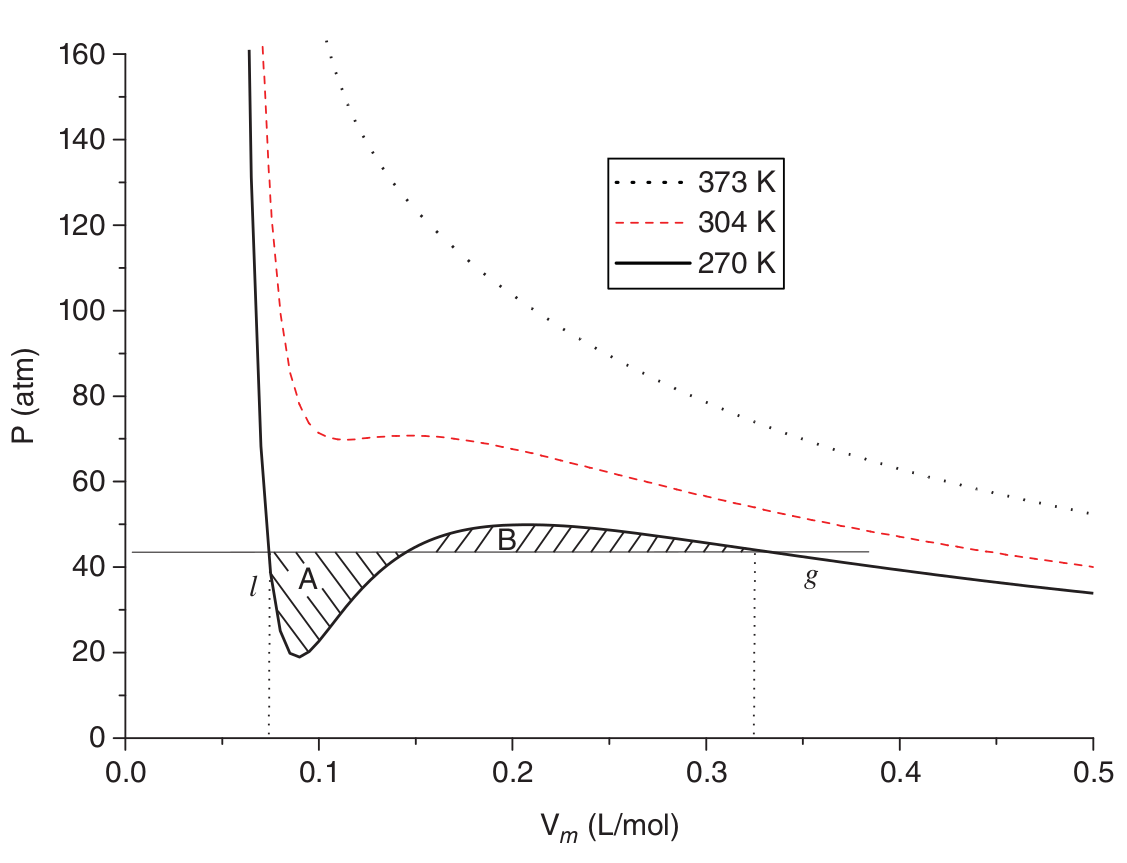
\includegraphics[width=.8\textwidth]{figs/cap2/Diagrama_P_V_del_CO2_Multiphase_LBM}
	\caption{Diagrama $P - V_m$ de la EOS de VdW del $CO_2$ con las constantes $a = 3,592$ y $b = 0,04267$, representando par a $T = 270 \> K$ los volúmenes molares del líquido y gas. \cite{huang2015multiphase}}
	\label{fig:P_V_CO2}	
\end{figure}


La EOS \ref{eq:VdW_P} se puede re-estructurar como \ref{eq:VdW_rho} puesto que $\rho = \frac{1}{v}$, siendo $v$ el volúmen másico y relacionando $V_m$ con $v$. Donde para un dado valor de temperatura tendremos la coexistencia de fases con su densidad $\rho_l$ para la fase líquida y $\rho_g$ para la gaseosa.

\begin{equation}
p = \frac{\rho R T}{1- \rho B} - A {\rho}^{2}
\label{eq:VdW_rho}
\end{equation}


%%% Local Variables: 
%%% mode: latex
%%% TeX-master: "template"
%%% End: 